\documentclass{article}

% Packages
\usepackage[utf8]{inputenc} % UTF-8 input encoding
\usepackage[T1]{fontenc} % Font encoding
\usepackage{amsmath, amssymb} % Math packages
\usepackage{enumitem} % For customizing lists
\usepackage{lipsum} % For generating dummy text
\usepackage{listings}
\usepackage{graphicx}


\lstset{%
  language=bash,
  basicstyle=\fontfamily{pcr}\selectfont,
  commentstyle=\bfseries,
  escapeinside={(*@}{@*)}
}

\newcommand{\comment}[1]{\# here is a comment: #1}
\newcommand\floor[1]{\lfloor#1\rfloor}
\newcommand\ceil[1]{\lceil#1\rceil}

% Title and author information
\title{Algorithms (6470) HW03a}
\author{Alex Darwiche}
\date{\today}

\begin{document}

\maketitle

\section*{Answers}

% Question 1
\subsection*{Q1}
\begin{enumerate}[label=(\alph*)]
    \item Find the optimal way to parenthisize matrices with dimenions: <9,3,8,2,5,6>
    \subitem 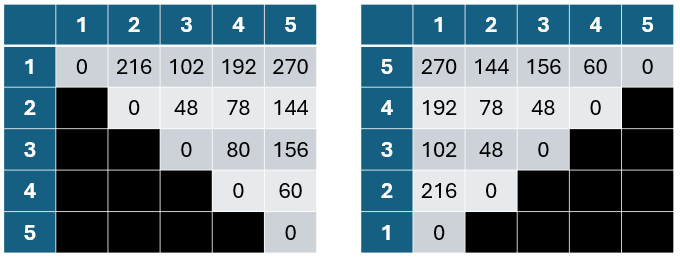
\includegraphics[width=1\textwidth]{tableM.png}
    \subitem 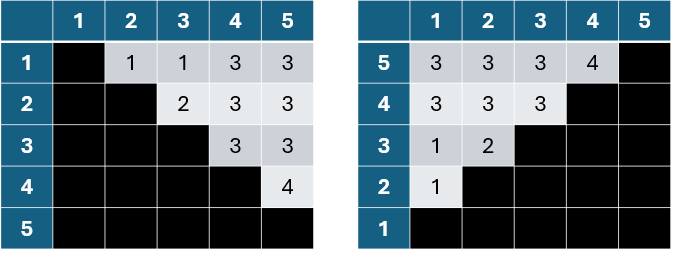
\includegraphics[width=1\textwidth]{tableS.png}

\end{enumerate}

% Question 2
\subsection*{Q2}
\begin{enumerate}[label=(\alph*)]
    \item To find the maximum total product of a subarray within A we can use the following logic. We first know that the array A has positive and negative integers. This means, that we need to keep track of both maximum and minimum values throughout our dynamic programming solution. The intuition for this will be that if we're trying to find the Maximum Product subarry of A, we can rewrite that as the maximum of 4 different elements:
    \subitem (1) A[1] 
    \subitem (2) MaxSubArrayOf(A[2:n])
    \subitem (3) A[1]*MaxSubArrayOf(A[2:n])
    \subitem (4) or A[1]*MinSubArrayOf(A[2:n])
    
    \item We can see here, how the larger problem can be broken down into smaller parts, by understanding that the Maximum Product is simply the maximum AND MINIMUM product of smaller arrays.
    \item Recurrence Relation
    \begin{lstlisting}[frame=single]
        MaxSubArray(A) = Max(
                            A[1], 
                            A[1]*MaxSubArray(A[2:n]), 
                            A[1]*MinSubArray(A[2:n]), 
                            MaxSubArray(A[2:n])
                            )
    \end{lstlisting}
    \item It is important to note that we keep track of the minimum of the sub arrays as well. This is because a negative times a negative is a positive number.
    \item Sample Psuedocode of an iterative solution
    \begin{lstlisting}[frame=single]
    def MaxSubArray(A):
        max = min = A[1]
        n = A.size()
        upper_bound_max = lower_bound_max = 1
        upper_bound_min = lower_bound_min = 1
        
        for i in 2 to n:
            // Update Max Values
            if (A[i] > max):
                lower_bound_max = i
                upper_bound_max = i
                max = A[i]
            else if (A[i]*max > max):
                upper_bound_max = i
                max = A[i]*max
            else if (A[i]*min > max):
                lower_bound_max = lower_bound_min
                upper_bound_max = i
                max = A[i]*min

            // Update Min Values
            else if (A[i] < min):
                lower_bound_min = i
                upper_bound_min = i
                min = A[i]
            else if (A[i]*max < min):
                lower_bound_min = lower_bound_max
                upper_bound_min = i
                min = A[i]*max
            else if (A[i]*min < min):
                upper_bound_min = i
                min = A[i]*min

        return max, lower_bound, upper_bound
    \end{lstlisting}
\end{enumerate}

% Question 3
\subsection*{Q3}
\begin{enumerate}[label=(\alph*)]
    \item This problem requires that we "convert" DISTANCE to DESTINY. This can be done using the bottom up approach where we determine the actions needed and fill out the following table.
    \item Recurrence Relation
    \begin{lstlisting}[frame=single]
        Assume A = "DISTANCE" and B = "DESTINY"

        if A[i] = B[j] then this is a match
            edit(i+1,j+1)
        if A[i] does not equal B[j]:
            1 + minimum(
                    edit(i, j+1) //Insertion
                    edit(i+1, j) //Deletion
                    edit(i+1,j+1) //Replacement    
                )
        \end{lstlisting}
    \item Table illustrating this process:
    \subitem 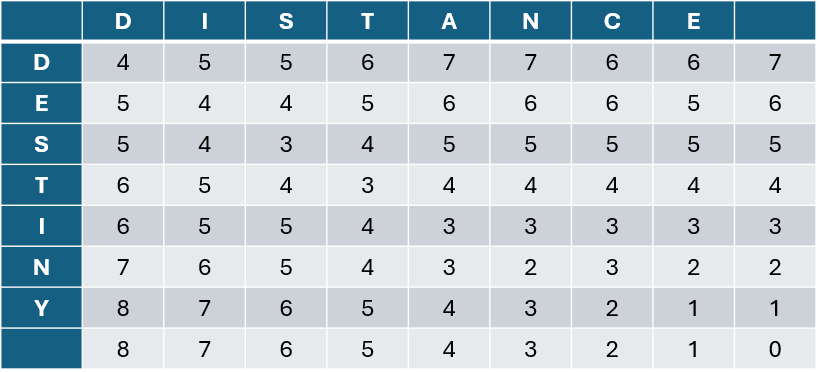
\includegraphics[width=1\textwidth]{editDistance.png}

    \item 4 total actions with 3 Replacements and 1 Deletion, along with 4 matches.
    \subitem Cost = $3*(-4) + (-2) + 4*(4) = +2$
\end{enumerate}

% Question 4 (Graduate students only)
\subsection*{Q1 (Graduate students only)}
\begin{enumerate}[label=(\alph*)]
    \item This problem asks us to find the min total perimeter of triangles in a triagulated convex polygon.
    \item The inuition for this will be to continually break down the polygon into smaller and smaller polygons until it is all triangles. Then you return the minimum perimeter after looking through all possible triangulations. 
    \item To do this, we find the minimum perimeter triangle between vertex i, j, and k. You Start by setting i to the first vertex and j to the last vertex. Then, k iterates from the vertex adjacent to i, until it is adjacent to j. We can splice a polygon into subpolygon and calculate the cost of all triangulations.
    \item 3 Vertices will always create a triangle. We want to find the perimeter of that triangle, and then find the triangles that describe the remaining polygons.
    \item As you can see in the following picture, there are 2 cases when splitting a polygon. You either create an edge triangle and a polygon, or you create a triangle and two polygons. Either way, the following psuedocode will work.
    \item In both cases, you calculate MinPerimeter(i,j) = MinPerimeter(i,k) + MinPerimeter(j,k) + Perimeter(i,j,k)
    \subitem 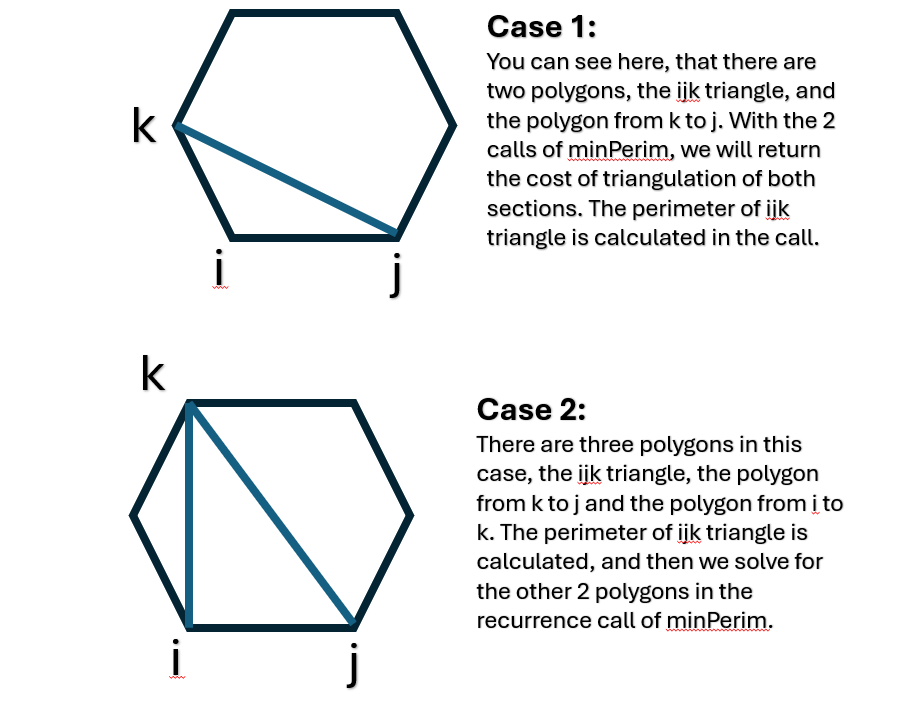
\includegraphics[width=1\textwidth]{polygon.png}
    \item Psuedocode
    \begin{lstlisting}[frame=single]
    # Use distance formula to calculate total cost
    def perimeter(i,j,k):
        return d(i,j) + d(i,k) + d(j,k)
    
    def minPerim(vertices, i, j):
        vertices = (x1,y1), (x2,y2)...(xN,yN)
        i = 1
        j = n

        # Base case vertices next to one another
        if i + 2 > j: 
            return 0
        
        # Next, find the min triangulation
        for k in i+1 to j:
            min = min(min, 
                minPerim(vertices, i, k) +
                minPerim(vertices, k, j) + 
                perimeter(i,j,k)
            )
        return min
        \end{lstlisting}
\end{enumerate}


\end{document}
